\section{Evaluation}
\label{sec:eval}
%
\begin{figure}[t!]
\begin{center}
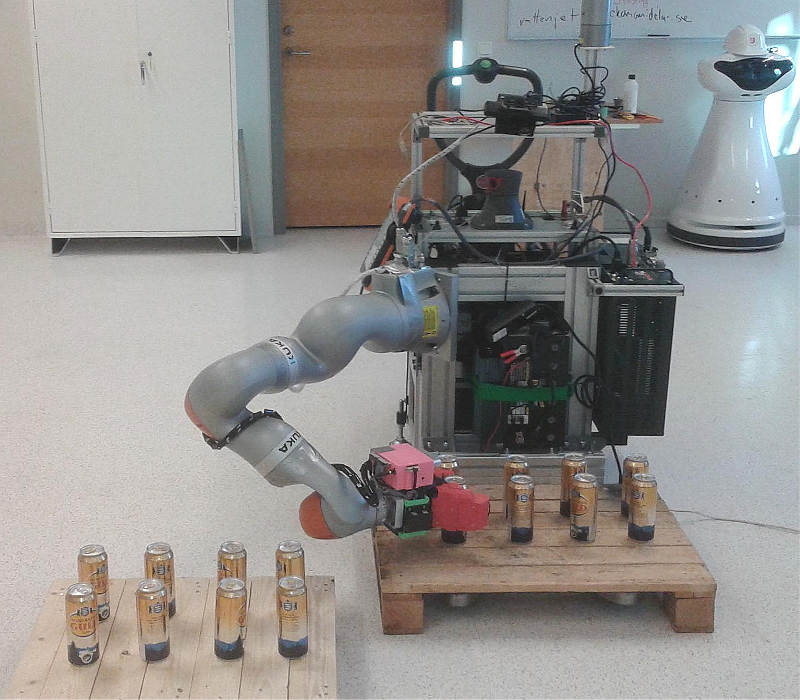
\includegraphics[width =1\linewidth]{figs/demo}
%\vspace{-0.25cm}
\caption{\textit{Demo setup:} The robot loads beer onto a previously picked up pallet and
  subsequently transports it to a predefined target location.}
\label{fig:demo_setup}
\vspace{-0.65cm}
\end{center}
\end{figure}
%
\hl{todo...}

\cite{Kano09} task function description; Used off-the-shelf
solver\footnote{\url{http://www.gurobi.com}} ROS\footnote{\url{http://www.ros.org/}}
